\documentclass[a4paper,12pt]{article}
\usepackage[backend=biber, citestyle=authoryear, bibencoding=utf8]{biblatex}
\addbibresource{proposal.bib}

\usepackage{amsmath, amsfonts}

\usepackage{pgf, tikz}
\usetikzlibrary{arrows, automata}


\DeclareMathOperator*{\argmax}{argmax}

\begin{document}

\subsection*{Counterfactual Analysis and Social Planners}

The social planner's problem consists of finding the global optimum, in terms of the aggregated utility of the population, over a given set of policies, conditional on a given set of covariates.
%
$$
\argmax_{\pi} \  h((u_1(\pi | X_1), u_2(\pi | X_2),\dots, u_n(\pi | X_N)))
$$

Where $h(\cdot)$ represents the aggregation function of interest for the policy maker and aggregates over the population of size $N$.

If there is only one policy in the optimization set, then finding the global optimum consists in choosing between the policy and the null set (the treatment and the control) given the covariates. If, additionally, the policy maker is interested in maximizing the total welfare of the population, then the problem reduces to
%
$$
\argmax_{\pi \in \{\pi_0, \pi_1\}} \ \sum_{i=0}^N u_i(\pi | X_i)
$$

We can split the covariate variables, $X$, into two parts, one containing variables that vary on an individual level and can be assumed to be I.I.D. across individuals ($W$) and another part consisting of all the variables which are not independent (at the simplest extreme, population variables which are literally identical across individuals) which we will call $Z$. This allows us to transform the maximization problem of total utility into one of expected utility:
%
$$
\argmax_{\pi \in \{\pi_0, \pi_1\}} \ \mathbb{E}_W \big[ u(\pi | Z) \big]
$$

Where the expectation operates over the individual-level I.I.D. variables $W_i$. Adopting the notation from the potential outcomes framework with utility substituted for generic outcome-of-interest $Y$, can be written as
%
$$
\begin{cases}
\pi_1, & \mathbb{E}\big[ Y^1 - Y^0 | Z \big] > 0 \\
\pi_0, & otherwise
\end{cases}
$$

Where $\mathbb{E}\big[ Y^1 - Y^0 | Z \big]$ is the conditional average treatment effect (CATE). The CATE can be estimated, using the weak law of large numbers, using a sample of independent observations of the treatment on the population of interest.
%
$$
\frac{1}{n} \sum_i Y_i | Z_i=z \ \overset{p}{\to} \ \mathbb{E}\big[ Y^1 - Y^0 | z \big]
$$

If $Z$, the non-I.I.D. variables, contains a variable for which there is not full support in the observations, then one cannot compute the CATE conditional on the unsupported state. In particular, if one naively models time as a set of discrete dummy variables that might interact with the treatment, then: 
%
$$
\frac{1}{n} \sum_i Y_i | Z_{i}=z_{t-1} \ \overset{p}{\not\to} \ \mathbb{E}\big[ Y^1 - Y^0 | z_t \big]
$$

The CATE is an evaluation of ceteris parabis counterfactual analysis. It tells us what would have happened, if everything else in the universe stayed exactly the same, except for the one bit of randomness that led an individual to be treated (or not). Counterfactual analysis, however, is not the social planner's question. The social planner's question is not the (interesting) legal and philosophical question about what would have happened in the past had a different decision been made. The social planner's question is what to do in the present in order to maximize some objective function. What would have happened in the past conditional on a given set of covariates is not the same as what will happen in the future conditional on a different set of covariates, and the conversion can only be made with full support in the past. 

What about the average treatment effect (ATE)? Can we compute the ATE and does this solve the social planner's problem? The ATE has two problems that make it an undesireable substitute:

\begin{enumerate}

\item Marginalizing out any given covariate requires integration over the entire range of its possible values. As before, any variable which is not independent in our observations, or that lacks full support in the observed data, makes this marginalization impossible.

\item The ATE is a more general formulation than the CATE in the social planners problem. This more general formulation is not only more difficult to estimate, requiring more data, but is also of less use to the social planner. If I am deciding whether or not to give a certain medication to my 6-month old child, not only do I not need to know the average effect of this medication on people of all ages (which would require data from a larger study than one on just 6-month olds), but I am also not likely to make my decision based on the average treatment effect of this medecine on persons of all ages, which can be arbitrarily far from the treatment effect on 6-month old babies.

\end{enumerate}

Given that both the CATE and the ATE are sample estimates that do not converge in probability to the population estimate of interest in our social planner's problem, is there a better estimate that can be made? In particular, what would qualify an estimate as the ``best'' answer to the social planner's question?

\subsection*{Expected Regret Minimization}

Let's return to the original, general formulation of the social planner's problem, with some lighter notation:
%
$$
\argmax_{\pi} \  h(\pi, X)
$$

We can formulate a reasonable goal of the social planner as that of minimizing their ``policy regret'':
%
$$
R_{\pi} = h(\pi^*, X) - h(\pi(X), X)
$$

Where $\pi^*$ represents the solution to the original maximization problem, the true best policy, and $\pi(\cdot)$ represents the function used by the social planner to choose their policy. We can decompose the covariates $X$ into two parts, one which contains random variables unknown to the social planner at the time of decision making ($W$) and the other which contains those variables that are known ($Z$). Given the random formulation, it can make sense for the social planner to want to minimize their expected policy regret:
%
$$
\mathbb{E}_W \big[ h(\pi^*, Z) - h(\pi(Z), Z)  \big]
$$

How can one find an estimate of an expectation over every unkown variable? With no further assumptions, $W$ needs to contain everything about the state of the entire world that could change from $t-1$ to $t$. Finding a sample estimate of that expectation would then require sampling from the entire distribution of everything in the world that could possibly change, while holding constant everything in the world we know will be constant.

We will make two simplifying assumptions in order to scope the problem more effectively:

\begin{enumerate}

\item That the aggregate utility of interest can be decomposed into a sum of two component parts:
%
$$
h(\pi, X) = g(\pi, B) + v(X)
$$

Where $B \subset X$ represents the covariates that interact in some way with the policy in question $\pi$. This assumptions means that some non-empty set of covariates, $X \setminus B$ affect the aggregate utility in a way which does not depend on the policy of interest. This allows us to rewrite the policy regret:
%
$$
R_{\pi} = g(\pi^*, B) - g(\pi(B), B)
$$

While this my seem like a formalize that has done nothing except introduce new variables, it is worthwhile to consider how we go from $X$ to $B$ in practise. Additionally, it is worth noting that $X \setminus B$ might contain variables that are useful in estimating a model of $g(\cdot)$, but do not actually need to be considered in the social planners optimization if they enter the objective function in a purely linear fashion. 

% YEAR FIXED EFFECTS AS A CONCRETE EXAMPLE??? 

\item Decompose the variables $B$ into their known quantities ($\phi$) and random quantities ($B \setminus \phi$). Then, we define a subset of the random variables unknown at time $t-1$, $\nu \subseteq (B \setminus \phi)$ as:
%
$$
p(g | \pi = \pi, \phi, \nu) = p(g | do(\pi := \pi), \phi, B \setminus \phi)
$$

\end{enumerate}

What we are left with then is the social planner's optimization problem in a more tractable form:
%
$$
\argmax_{\pi} \ \mathbb{E}_{\nu} \big[ g(\pi, \phi) \big]
$$

Where what we need is an expectation over all of our unknown quantities $\nu$, conditional on the known quantities $\phi$ and the policy $\pi$. This gives us a clear directive for the empirical work necessary to estimate the best solution to the social planner's problem. 

From assumption 2, we have that $g | \pi, \phi, \nu$ is invariant with respect to interventions $do(\pi := \pi)$, representing an independent causal mechanism. To calculate the expected regret, $\nu$ represents the exact set variables we must be able to marginalize out of our empirical regret estimates, and $\phi$ the exact set of variables we must know. 

Assumption 1 allows us to ignore all of the original, universal covariates that are not part of $B$. Again, while these variables might be useful in building a model of $g$ from empirical data, we neither need to know their value at time $t$ nor do we need to marginalize them out of our expected regret calculation. 

\subsection*{Example}

To take an example of where counterfactual analysis might differ from expected regret minimization, consider the following example which consists of four variables, in which one might think to use time fixed effects in a standard OLS regression: 

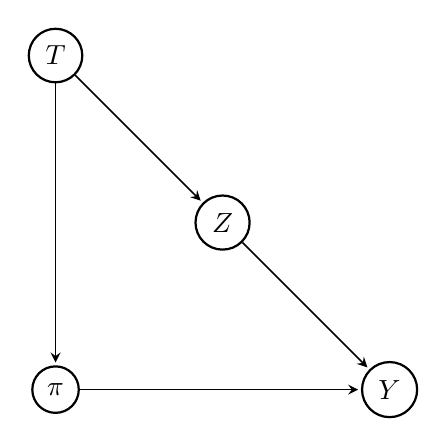
\begin{tikzpicture}[
  > = stealth, 
  shorten > = 1pt,
  auto,
  node distance = 3cm, 
  semithick 
  ]

  \tikzstyle{every state}=[
  draw = black,
  thick,
  fill = white,
  minimum size = 4mm
  ]

  \node[state] (t) {$T$};
  \node[state] (z) [below right of=t] {$Z$};
  \node[state] (x) [below left of=z] {$\pi$};
  \node[state] (y) [below right of=z] {$Y$}; 

  \path[->] (t) edge node {}(z);
  \path[->] (t) edge node {}(x);
  \path[->] (z) edge node {}(y);
  \path[->] (x) edge node {}(y);

\end{tikzpicture}


Where $Z$ represents a latent variable, or set of latent variables, that affects the outcome and changes over time. Because the treatment is also changed over time, these can cause confounding effects. One can block the confounding path by conditioning on the time, $T$, which can be done, for example, by conditioning on time dummy variables (time fixed effects) if one wants to allow the variables to be completely independent from one period to the next.

In counterfactual analysis, it should be clear that conditioning on $T$ is enough to recover the CATE, $\mathbb{E} \big[ Y^1 - Y^0 \big | Z ]$. However, in expected regret minimization, we would need to take an extra step in showing that either: 

\begin{enumerate}

\item The outcome $Y$, or its aggregation function $g$, is effected by $Z$ linearly of $\pi$, thus the effect of $Z$ at time $t$ is irrelevant for choosing the best policy $\pi$ and can be excluded. In other words, there is no interaction between the latent variables and the policy on the outcome.

\item $Z$ can be marginalized out of the conditional average treatment effect. This would be the case if the variables were I.I.D. In practise, one can imagine this is possible only when the correlation over time is weak enough and the number of time periods is large enough, such the number of effective samples grows large enough to approximate the whole distribution via the time-correlated observations and they are marginalized out in the sample average.

\end{enumerate}



\printbibliography
\end{document}
